  \section{Unidade de Processamento}

    \subsection{Diagrama de Classe}
      \begin{figure}[H]
      \centering
            \begin{tikzpicture} 
        \umlclass[type=control]{Processing\_Unit}
        { % atributos
          + clock : input bit \\
          + reset : input bit \\
          + data\_a : input bit[8] \\
          + data\_b : input bit[8] \\
          + operation : input bit[TBD] \\          
          + result\_data : output bit[8] \\
          + overflow : output bit \\
          - enable\_result\_reg : reg bit \\
          - reult\_reg : reg bit[8]
        }{ % procedures
          - \underline{<<comb>> process\_operation()} \\
          - <<comb>> setup\_flag() \\
          - <<sequ>> result\_reg\_handler()
        }
      \end{tikzpicture}
    \end{figure}

    \subsection{Definições de Entrada e Saída}
      \FloatBarrier
      \begin{center}
        \begin{longtable}[pos]{| l | c | c | m{7cm} |} \hline         
          \multicolumn{1}{|c|}{\cellcolor[gray]{0.9}\textbf{Nome}} & 
          \multicolumn{1}{c|}{\cellcolor[gray]{0.9}\textbf{Tamanho}} & 
          \multicolumn{1}{c|}{\cellcolor[gray]{0.9}\textbf{Direção}} &
          \multicolumn{1}{c|}{\cellcolor[gray]{0.9}\textbf{Descrição}} \\ \hline
          \endfirsthead
          \hline
          \multicolumn{4}{|l|}%
          {{\bfseries continuação da página anterior}} \\
          \hline
          \multicolumn{1}{|c|}{\cellcolor[gray]{0.9}\textbf{Nome}} & 
          \multicolumn{1}{c|}{\cellcolor[gray]{0.9}\textbf{Tamanho}} & 
          \multicolumn{1}{c|}{\cellcolor[gray]{0.9}\textbf{Direção}} &
          \multicolumn{1}{c|}{\cellcolor[gray]{0.9}\textbf{Descrição}} \\ \hline
          \endhead

          \multicolumn{4}{|r|}{{continua na próxima página}} \\ \hline
          \endfoot

          \hline
          \endlastfoot

          clock\_in                & 1   & entrada   & Clock principal do sistema.    \\ \hline
          reset\_in                & 1   & entrada   & Sinal de reset geral do sistema.    \\ \hline
          data\_a\_in              & 8   & entrada   & Dado do primeiro operando.    \\ \hline
          data\_b\_in              & 8   & entrada   & Dado do segundo operando.    \\ \hline
          operation\_in            & TBD   & entrada   & Código da operação.    \\ \hline
          result\_data\_out        & 8   & saída     & Representação do resultado da operação. \\ \hline
          overflow\_out            & 1   & saída     & Sinal indicador de overflow aritmético. \\
        \end{longtable}
      \end{center} 

    \subsection{Datapath Interno}
      \begin{figure}[H]
        \centering
        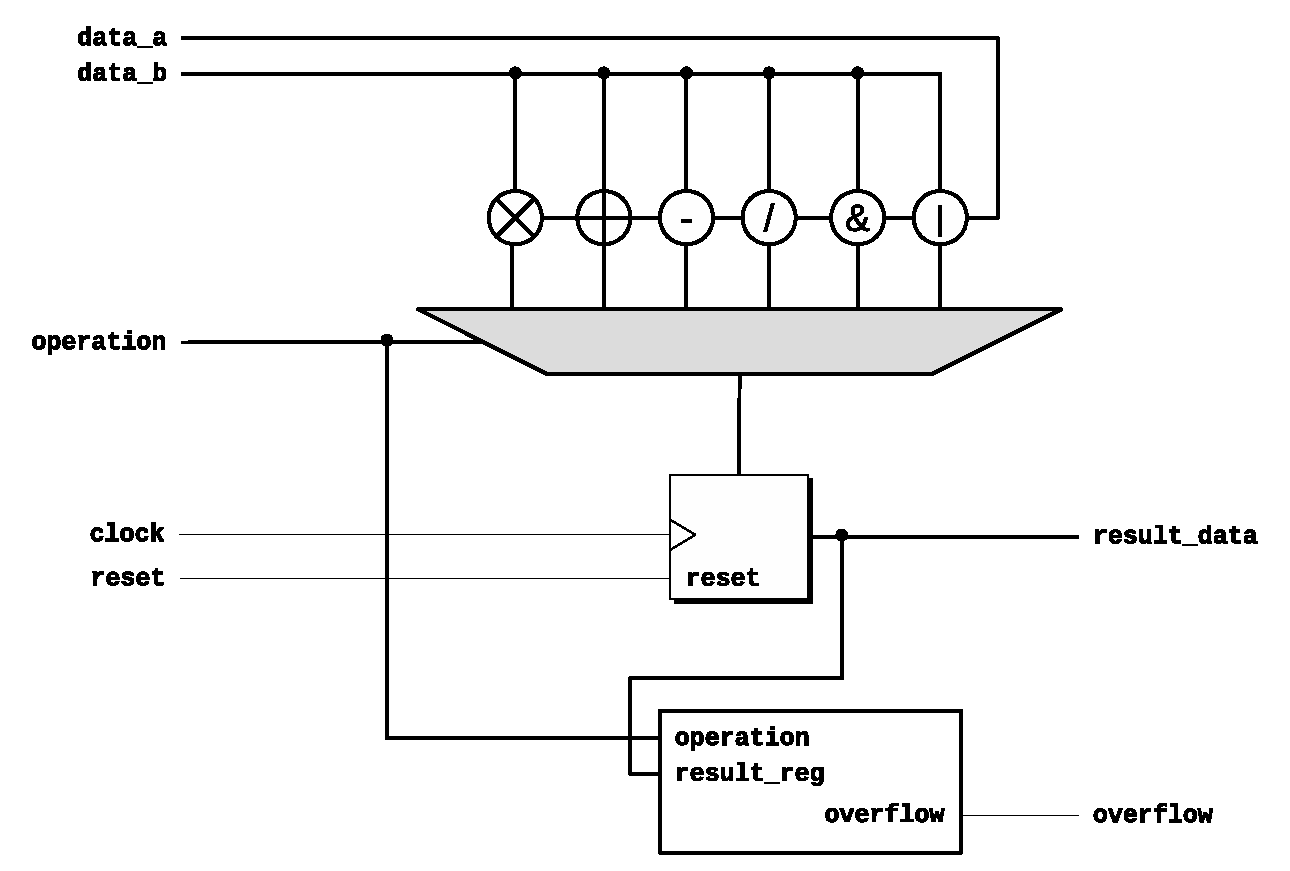
\includegraphics[width=\linewidth]{datapath/processing_datapath.eps}
      \end{figure}
    \newpage